\chapter{Desarrollo}

\section{Parámetros eléctricos del rectificador monofásico controlado}

Un sistema monofásico controlado a diferencia de un rectificador en base a diodos usa un SCR o tiristor que limita el paso de la señal a rectificar hasta que su puerto o gate es excitada con un voltaje de activación y cuya magnitud es dependiente al tipo de dispositivo.

En la figura \ref{fig:rec-controlado-monofasico} se muestra un circuito rectificador a media onda tradicional y que esta compuesto por una señal sinusoidal de entrada, el SCR y la salida o carga resistiva.

% TODO: \usepackage{graphicx} required
\begin{figure}[h]
	\centering
	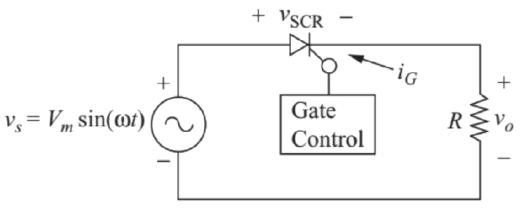
\includegraphics[width=0.7\linewidth]{media/rec-controlado-monofasico}
	\caption{Rectificador monofásico controlado}
	\label{fig:rec-controlado-monofasico}
\end{figure}

Para determinar el comportamiento eléctrico del circuito rectificador se debe hacer un análisis de forma similar a un rectificador tradicional con el leve cambio de que ahora por defecto se tendrá que tener en cuenta un \textbf{angulo de disparo} y que se encuentra en relación directa con el instante en el cual se decide excitar la puerta del SCR durante la excursión positiva de la señal de entrada.

De ello se obtiene las siguientes ecuaciones: 

\begin{align}
	V_{dc} &= \frac{V_m}{2\pi} (1 + \cos\alpha) \\
	I_{dc} &= \frac{V_m}{2\pi R} (1 + \cos\alpha) \\
	V_{rms} &= \frac{V_m}{2} \sqrt{ \pi - \alpha + \frac{\sin 2\alpha}{2} } \\	
	I_{rms} &= \frac{V_m}{2R} \sqrt{ \pi - \alpha + \frac{\sin 2\alpha}{2} } \\
	P 	&= \frac{V_{rms}^2}{R}
\end{align}

Que describen la relación de:

\begin{enumerate}
	\item Voltaje y corriente media
	\item Voltaje y corriente eficaz o RMS
	\item Potencia en la carga
\end{enumerate}

En función del angulo $\alpha$ el cual define el comportamiento del rectificador respecto a sus parámetros eléctricos.












